\documentclass[12pt,a4paper]{report}

\usepackage[utf8]{inputenc}
\usepackage[T1]{fontenc}
\usepackage[french]{babel}
\usepackage{geometry}
\geometry{margin=25mm}
\usepackage{graphicx}
\usepackage{array}
\usepackage{booktabs}
\usepackage{longtable}
\usepackage{tabularx}
\usepackage{enumitem}
\usepackage{xcolor}
\usepackage{tikz}
\usepackage{tcolorbox}
\usepackage{hyperref}
\usepackage{fancyhdr}
\usepackage{float}
\usepackage{ragged2e}
\usepackage{titlesec}
\usepackage{subcaption}
\usepackage{colortbl}

\usetikzlibrary{positioning,arrows.meta,calc,shapes.geometric}

\definecolor{proctorpurple}{HTML}{6200EE}
\definecolor{proctorred}{HTML}{B00020}
\definecolor{emsigreen}{HTML}{27AE60}
\definecolor{darkblue}{HTML}{1A5276}
\definecolor{darkgray}{HTML}{34495E}

\hypersetup{
  colorlinks=true,
  linkcolor=darkblue,
  urlcolor=proctorpurple,
  citecolor=darkblue,
  pdftitle={Rapport Gestion Charite},
  pdfauthor={GitHub Copilot}
}

\pagestyle{fancy}
\fancyhf{}
\lhead{Gestion Charite}
\rhead{Rapport technique}
\cfoot{\thepage}

\setlength{\parindent}{0pt}
\setlength{\parskip}{0.7em}
\renewcommand{\baselinestretch}{1.2}
\renewcommand{\arraystretch}{1.2}

\titleformat{\chapter}[display]
  {\normalfont\Huge\bfseries\color{darkblue}}{\chaptertitlename\ \thechapter}{20pt}{\Huge}
\titleformat{\section}{\Large\bfseries\color{emsigreen}}{\thesection}{1em}{}
\titleformat{\subsection}{\large\bfseries\color{darkgray}}{\thesubsection}{1em}{}

\definecolor{emsiblue}{HTML}{0B4F8A}
\definecolor{emsigold}{HTML}{F0B323}
\definecolor{softbg}{HTML}{F7F9FC}
\definecolor{cardline}{HTML}{D7E0EA}

\newcommand{\EMSILogo}{%
  \begin{tikzpicture}[baseline=(logo.base)]
    \node[rounded corners=10pt, fill=emsiblue, minimum width=4.3cm, minimum height=1.8cm, inner sep=0pt] (logo) {};
    \draw[fill=emsigold, draw=none] (-1.7,0.52) -- (-1.15,1.2) -- (-0.6,0.52) -- (-1.15,-0.1) -- cycle;
    \draw[fill=white, draw=none] (-0.95,0.52) -- (-0.4,1.2) -- (0.15,0.52) -- (-0.4,-0.1) -- cycle;
    \draw[fill=emsigold, draw=none] (0.05,0.52) -- (0.6,1.2) -- (1.15,0.52) -- (0.6,-0.1) -- cycle;
    \node[white, font=\bfseries\Huge] at (0.95,0.05) {EMSI};
  \end{tikzpicture}%
}

\newcommand{\screenframe}[3]{%
\begin{tikzpicture}[x=1cm,y=1cm, font=\sffamily]
  \draw[rounded corners=10pt, line width=0.8pt, fill=white, draw=cardline] (0,0) rectangle (12,7);
  \fill[emsiblue] (0,6.25) rectangle (12,7);
  \fill[emsigold] (0,6.25) rectangle (0.24,7);
  \node[white, anchor=west, font=\bfseries\large] at (0.45,6.65) {#1};
  \node[anchor=north west, align=left, text width=11.1cm] at (0.45,5.95) {#2};
  #3
\end{tikzpicture}%
}

\begin{document}

\begin{titlepage}
  \begin{flushright}
    \EMSILogo
  \end{flushright}
  \vspace{0.9cm}
  \begin{center}
    {\large \textbf{RAPPORT DU PROJET DE FIN D'ETUDES}\par}
    \vspace{0.8cm}
    {\Huge\bfseries\color{darkblue} GESTION CHARITE\par}
    \vspace{0.6cm}
    {\Large Plateforme web de gestion des organisations, actions, dons et participations\par}
    \vspace{1cm}
    {\large \textbf{Modules:} Frontend React, Gestion de projet et Entrepreneuriat\par}
    \vspace{0.7cm}
    {\large \textbf{Technologies:} React, TypeScript, Spring Boot, MongoDB, Docker\par}
    \vspace{1cm}
    \begin{tcolorbox}[colback=softbg,colframe=cardline,boxrule=0.7pt,arc=6pt,width=0.9\textwidth]
      \centering
      \textbf{Réalisé par :} Équipe projet Gestion Charite\\[0.3cm]
      \textbf{Encadrement :} Projet académique EMSI\\[0.3cm]
      \textbf{Année universitaire :} 2025/2026
    \end{tcolorbox}
  \end{center}
\end{titlepage}

\pagenumbering{roman}

\chapter*{Dédicaces}
\addcontentsline{toc}{chapter}{Dédicaces}
Ce travail est dédié à nos parents, à notre entourage proche et à toutes les personnes qui ont soutenu cette réalisation depuis ses premières étapes.

\newpage
\chapter*{Remerciements}
\addcontentsline{toc}{chapter}{Remerciements}
Nous adressons nos remerciements à l'encadrement académique, aux enseignants et à toutes les personnes qui ont contribué à ce projet par leurs conseils, leur disponibilité et leurs retours.

\newpage
\chapter*{Résumé}
\addcontentsline{toc}{chapter}{Résumé}
Gestion Charite est une plateforme web dédiée à la gestion des organisations caritatives, des actions solidaires, des dons et de la participation. Le projet associe un frontend React, un backend Spring Boot, une base MongoDB et une couche d'administration pour le contrôle et la supervision des contenus.

\textbf{Mots-clés :} charité, React, Spring Boot, MongoDB, administration, organisation, dons, participation.

\newpage
\chapter*{Abstract}
\addcontentsline{toc}{chapter}{Abstract}
Gestion Charite is a web platform dedicated to managing charities, solidarity actions, donations and participation workflows. The project combines a React frontend, a Spring Boot backend, a MongoDB database and an administrative layer used for validation and supervision.

\textbf{Keywords:} charity, React, Spring Boot, MongoDB, administration, organization, donations, participation.

\newpage
\chapter*{Liste des Abréviations}
\addcontentsline{toc}{chapter}{Liste des Abréviations}
\begin{itemize}[label=\textbullet, itemsep=8pt]
  \item \textbf{API :} Application Programming Interface
  \item \textbf{CRUD :} Create, Read, Update, Delete
  \item \textbf{DTO :} Data Transfer Object
  \item \textbf{JWT :} JSON Web Token
  \item \textbf{MVC :} Model-View-Controller
  \item \textbf{MVVM :} Model-View-ViewModel
  \item \textbf{NoSQL :} Not Only SQL
  \item \textbf{REST :} Representational State Transfer
  \item \textbf{UI :} User Interface
  \item \textbf{UML :} Unified Modeling Language
\end{itemize}

\newpage
\listoffigures
\addcontentsline{toc}{chapter}{Liste des Figures}

\newpage
\listoftables
\addcontentsline{toc}{chapter}{Liste des Tableaux}

\newpage
\tableofcontents
\clearpage

\cleardoublepage
\pagenumbering{arabic}

\chapter*{Introduction Générale}
\addcontentsline{toc}{chapter}{Introduction Générale}
La plateforme \textit{Gestion Charite} est une application web complète destinée à centraliser la gestion des organisations, des actions caritatives, des dons, de la participation et de l'administration.
Le projet combine un frontend moderne en React avec un backend Spring Boot et une base MongoDB.

Au-delà d'une simple interface de consultation, la solution a été pensée comme un système de gestion complet. Elle doit permettre à un visiteur de comprendre rapidement les campagnes actives, à un donneur de contribuer en quelques étapes, à un organisateur de piloter ses actions, et à un administrateur de contrôler la qualité et la cohérence des données.

Le rapport s'appuie volontairement sur plusieurs formes de documentation visuelle. Les diagrammes UML décrivent la structure fonctionnelle du système, tandis que les captures d'écran montrent le comportement réel de l'application et les pages principales réellement utilisées dans le flux de travail.

Ce rapport est organise en trois modules:
\begin{itemize}[leftmargin=1.2cm]
  \item le module \textbf{Frontend React}, qui couvre l'experience utilisateur et les ecrans principaux;
  \item le module \textbf{Gestion de projet}, qui resume la conduite du projet, l'organisation du travail et la validation;
  \item le module \textbf{Entrepreneuriat}, qui met en avant la valeur ajoutee, les utilisateurs cibles et l'impact du produit.
\end{itemize}

\chapter{Module 1 - Frontend React}

\section{Objectif}
Le frontend a pour rôle de fournir une interface claire, responsive et accessible pour les visiteurs, donateurs, organisateurs et administrateurs.
Il consomme les services backend via l'API REST et affiche les donnees en temps reel, avec un accent sur la lisibilite des formulaires, la navigation et les retours utilisateur.

\section{Architecture fonctionnelle}
Les principaux blocs du frontend sont les suivants:
\begin{itemize}[leftmargin=1.2cm]
  \item la navigation generale et le layout applicatif;
  \item les pages d'authentification et de profil;
  \item le tableau de bord organisateur;
  \item la page d'administration;
  \item les formulaires de don, de participation et de gestion des actions.
\end{itemize}

\section{Parcours utilisateur}
Le parcours standard commence par la page d'accueil ou d'authentification, puis continue vers la consultation des actions, le don, la participation ou l'acces au dashboard selon le role.
Les composants React utilisent des hooks de service pour separer l'interface de la logique d'acces API.

Dans la pratique, la navigation a été organisée pour réduire le nombre d'étapes nécessaires entre la découverte d'une campagne et l'action utilisateur. Le visiteur voit les contenus publics, le donneur accède à des formulaires orientés conversion, et l'organisateur dispose d'écrans de gestion centrés sur l'opérationnel.

\section{Ecrans de l'application}
Les figures suivantes ne sont pas des captures brutes d'écran, mais des maquettes fidèlement inspirées des pages de l'application pour documenter l'interface.

Elles servent à présenter la logique visuelle de l'application avant d'introduire les captures réelles, qui montrent ensuite les écrans exécutés dans le navigateur.

\begin{figure}[H]
  \centering
  \screenframe{Ecran de connexion}{
    Connexion pour visiteur, donneur, organisateur ou super-admin.\par
    Authentification locale et Google OAuth selon le profil.
  }{%
    \draw[rounded corners=4pt, fill=softbg, draw=cardline] (0.7,4.35) rectangle (5.3,5.0);
    \node[anchor=west] at (0.95,4.675) {Email};
    \draw[rounded corners=4pt, fill=white, draw=cardline] (0.7,3.3) rectangle (5.3,3.95);
    \node[anchor=west] at (0.95,3.625) {Mot de passe};
    \draw[rounded corners=7pt, fill=emsigold, draw=none] (0.7,2.05) rectangle (3.3,2.7);
    \node[white, font=\bfseries] at (2.0,2.38) {Se connecter};
    \draw[rounded corners=7pt, fill=emsiblue!12, draw=emsiblue] (3.6,2.05) rectangle (5.3,2.7);
    \node[emsiblue, font=\bfseries] at (4.45,2.38) {Google};
  }
  \caption{Maquette de l'écran de connexion.}
\end{figure}

\begin{figure}[H]
  \centering
  \screenframe{Page d'exploration}{
    Consultation des actions caritatives disponibles, filtres par categorie et visualisation rapide des campagnes.
  }{%
    \draw[rounded corners=4pt, fill=softbg, draw=cardline] (0.7,4.6) rectangle (2.7,5.3);
    \draw[rounded corners=4pt, fill=softbg, draw=cardline] (3.0,4.6) rectangle (5.0,5.3);
    \draw[rounded corners=4pt, fill=softbg, draw=cardline] (5.3,4.6) rectangle (7.3,5.3);
    \draw[rounded corners=6pt, fill=white, draw=cardline] (0.7,2.5) rectangle (3.4,4.1);
    \draw[rounded corners=6pt, fill=white, draw=cardline] (3.7,2.5) rectangle (6.4,4.1);
    \draw[rounded corners=6pt, fill=white, draw=cardline] (6.7,2.5) rectangle (9.4,4.1);
    \draw[rounded corners=6pt, fill=emsigold, draw=none] (0.9,2.75) rectangle (1.7,3.05);
    \draw[rounded corners=6pt, fill=emsigold, draw=none] (4.0,2.75) rectangle (4.8,3.05);
    \draw[rounded corners=6pt, fill=emsigold, draw=none] (7.0,2.75) rectangle (7.8,3.05);
  }
  \caption{Maquette de la page d'exploration.}
\end{figure}

\begin{figure}[H]
  \centering
  \screenframe{Dashboard organisateur}{
    Suivi des actions, edition de l'organisation, et vue synthese des dons et participations.
  }{%
    \draw[rounded corners=6pt, fill=softbg, draw=cardline] (0.7,4.3) rectangle (2.5,5.2);
    \draw[rounded corners=6pt, fill=softbg, draw=cardline] (2.8,4.3) rectangle (4.6,5.2);
    \draw[rounded corners=6pt, fill=softbg, draw=cardline] (4.9,4.3) rectangle (6.7,5.2);
    \draw[rounded corners=6pt, fill=white, draw=cardline] (0.7,1.1) rectangle (9.4,3.7);
    \draw[fill=emsiblue!8, draw=cardline] (0.95,3.2) rectangle (9.1,3.5);
    \draw[fill=emsiblue!8, draw=cardline] (0.95,2.6) rectangle (9.1,2.9);
    \draw[fill=emsiblue!8, draw=cardline] (0.95,2.0) rectangle (9.1,2.3);
  }
  \caption{Maquette du dashboard organisateur.}
\end{figure}

\begin{figure}[H]
  \centering
  \screenframe{Dashboard admin}{
    Validation des organisations, pilotage global et supervision des comptes et des dons.
  }{%
    \draw[rounded corners=6pt, fill=softbg, draw=cardline] (0.7,4.3) rectangle (2.5,5.2);
    \draw[rounded corners=6pt, fill=softbg, draw=cardline] (2.8,4.3) rectangle (4.6,5.2);
    \draw[rounded corners=6pt, fill=softbg, draw=cardline] (4.9,4.3) rectangle (6.7,5.2);
    \draw[rounded corners=6pt, fill=softbg, draw=cardline] (7.0,4.3) rectangle (9.4,5.2);
    \draw[rounded corners=6pt, fill=white, draw=cardline] (0.7,1.1) rectangle (9.4,3.7);
    \draw[fill=emsigold!25, draw=cardline] (0.95,3.15) rectangle (9.1,3.48);
    \draw[fill=emsigold!25, draw=cardline] (0.95,2.5) rectangle (9.1,2.83);
    \draw[fill=emsigold!25, draw=cardline] (0.95,1.85) rectangle (9.1,2.18);
  }
  \caption{Maquette du dashboard administrateur.}
\end{figure}

\section{Diagrammes du frontend et du systeme}
Les diagrammes ci-dessous documentent les flux principaux du systeme, depuis le parcours utilisateur jusqu'aux traitements de donation et d'administration.

Chaque diagramme a un rôle précis: les cas d'utilisation clarifient les rôles et les responsabilités, le diagramme de classes structure les entités métier, le diagramme d'activité décrit un scénario de modification, et les séquences montrent les échanges successifs entre l'utilisateur et les services backend.

\begin{figure}[H]
  \centering
  
\includegraphics[width=\textwidth]{docs/diagrams/use_case_public.pdf}
  \caption{Cas d'utilisation public et organisateur.}
\end{figure}

\begin{figure}[H]
  \centering
  
\includegraphics[width=\textwidth]{docs/diagrams/use_case_admin.pdf}
  \caption{Cas d'utilisation administrateur.}
\end{figure}

\begin{figure}[H]
  \centering
  
\includegraphics[width=\textwidth]{docs/diagrams/class.pdf}
  \caption{Diagramme de classes principal.}
\end{figure}

\begin{figure}[H]
  \centering
  
\includegraphics[width=\textwidth]{docs/diagrams/activity.pdf}
  \caption{Diagramme d'activite pour la modification d'organisation.}
\end{figure}

\begin{figure}[H]
  \centering
  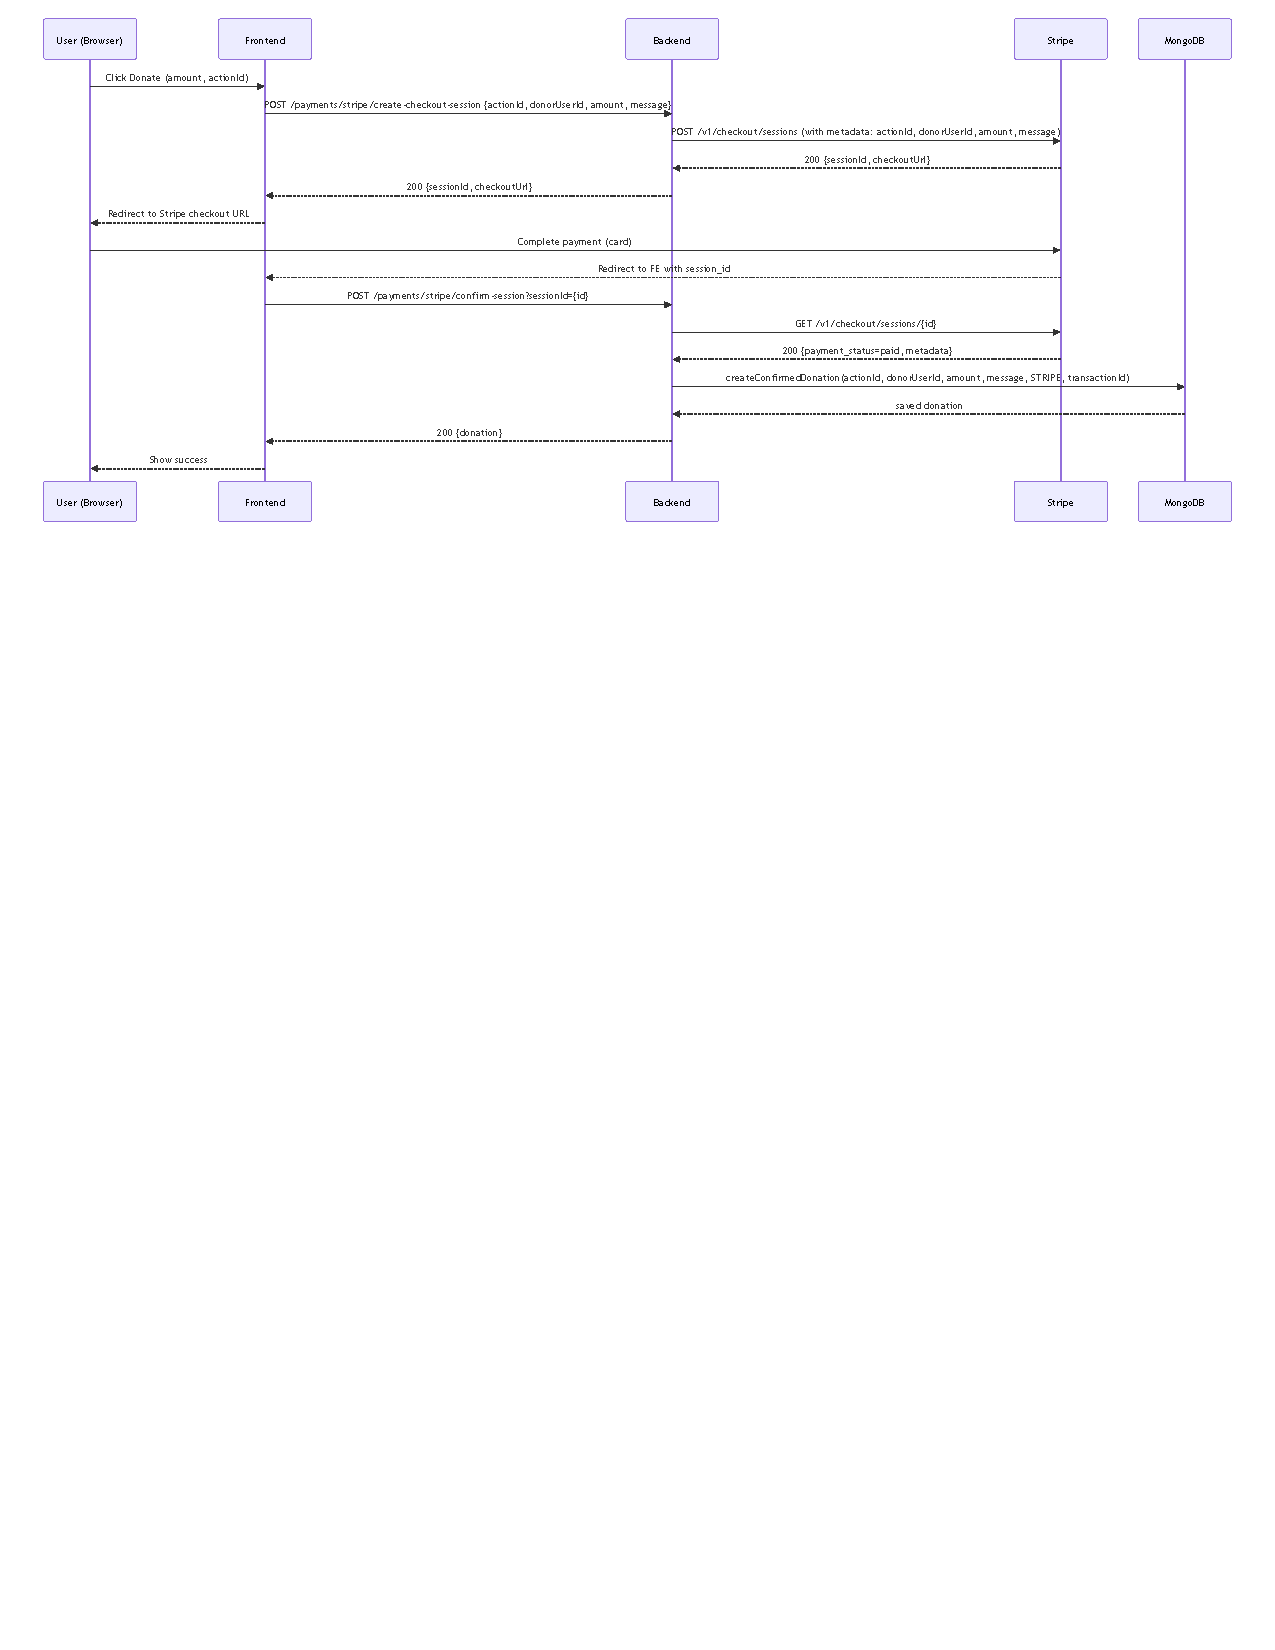
\includegraphics[width=\textwidth]{docs/diagrams/donation_sequence.pdf}
  \caption{Sequence de donation.}
\end{figure}

\begin{figure}[H]
  \centering
  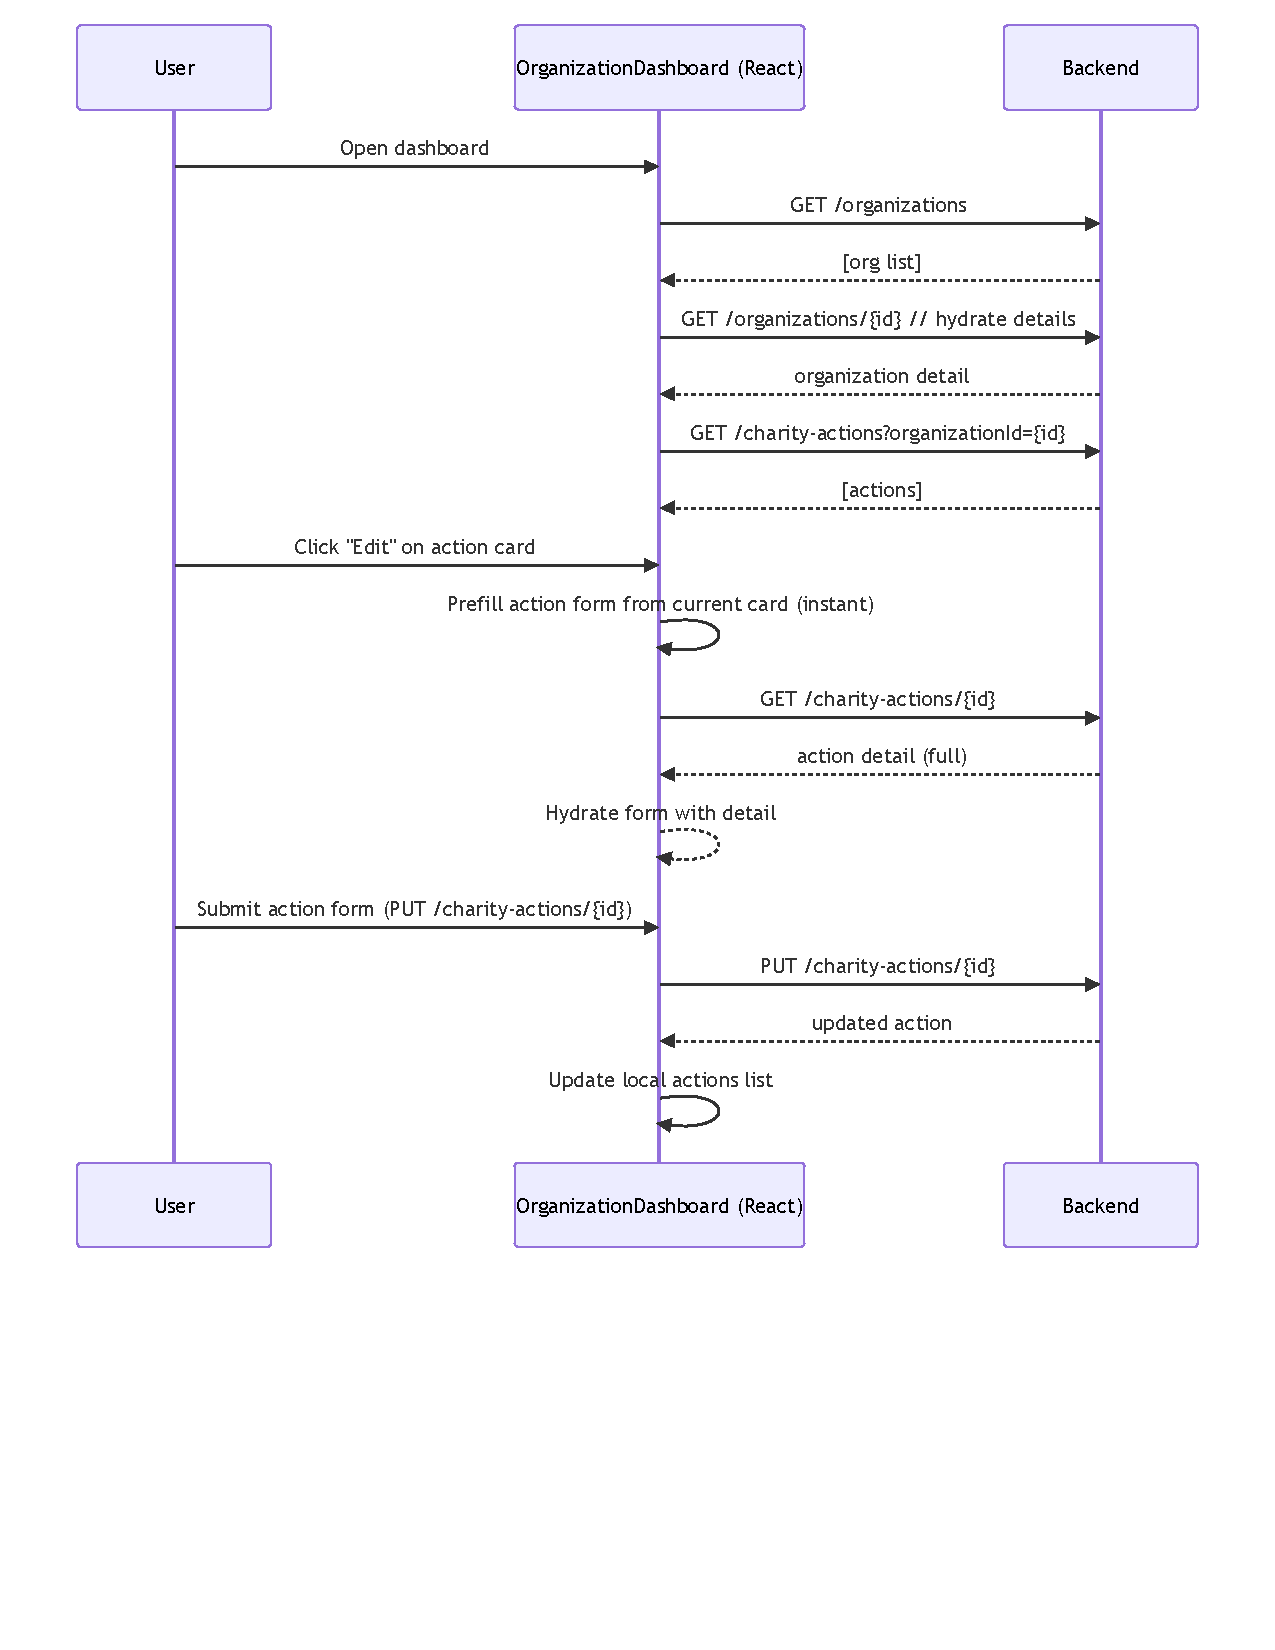
\includegraphics[width=\textwidth]{docs/diagrams/org_sequence.pdf}
  \caption{Sequence de modification du dashboard organisation.}
\end{figure}

\chapter{Captures réelles de l'application}

\section{Principe de documentation visuelle}
Les captures ci-dessous ont été réalisées à partir de l'application en fonctionnement ou, lorsque cela était nécessaire pour le back-office, à partir des templates d'administration fournis dans le projet. Elles complètent les maquettes en montrant le rendu final et les principaux états d'interface utilisés dans l'application.

\section{Frontend public et utilisateur}
Cette première série illustre le parcours standard d'un utilisateur: connexion, consultation, don, suivi du profil et découverte des organisations.

\subsection{Écran de connexion}
Cet écran matérialise l'entrée dans la plateforme et le choix du mode d'accès selon le profil de l'utilisateur.
\begin{figure}[H]
  \centering
  \includegraphics[width=0.92\textwidth]{docs/screenshots/01-auth-login.png}
  \caption{Capture réelle de l'écran de connexion.}
\end{figure}

\subsection{Dashboard donneur}
Après authentification, le tableau de bord synthétise l'activité de l'utilisateur et propose des accès rapides aux fonctionnalités principales.
\begin{figure}[H]
  \centering
  \includegraphics[width=0.92\textwidth]{docs/screenshots/02-dashboard-donor.png}
  \caption{Capture réelle du dashboard donneur.}
\end{figure}

\subsection{Exploration des actions}
Cette vue montre la page de découverte des campagnes, avec filtres et cartes d'actions caritatives.
\begin{figure}[H]
  \centering
  \includegraphics[width=0.92\textwidth]{docs/screenshots/03-explore.png}
  \caption{Capture réelle de la page d'exploration.}
\end{figure}

\subsection{Formulaire de don}
La page de don détaille le montant, l'action ciblée et le parcours de confirmation avant enregistrement du versement.
\begin{figure}[H]
  \centering
  \includegraphics[width=0.92\textwidth]{docs/screenshots/04-donate.png}
  \caption{Capture réelle de la page de don.}
\end{figure}

\subsection{Profil utilisateur}
Le profil rassemble les informations personnelles et les indicateurs liés aux contributions de l'utilisateur.
\begin{figure}[H]
  \centering
  \includegraphics[width=0.92\textwidth]{docs/screenshots/05-profile.png}
  \caption{Capture réelle de la page profil.}
\end{figure}

\subsection{Participation}
Cette interface présente la participation à une action et le suivi des engagements pris dans la plateforme.
\begin{figure}[H]
  \centering
  \includegraphics[width=0.92\textwidth]{docs/screenshots/06-participate.png}
  \caption{Capture réelle de la page participer.}
\end{figure}

\subsection{Organisation}
Cette vue décrit l'organisation associée au compte courant et les éléments disponibles pour l'utilisateur.
\begin{figure}[H]
  \centering
  \includegraphics[width=0.92\textwidth]{docs/screenshots/07-organization.png}
  \caption{Capture réelle de la page organisation.}
\end{figure}

\section{Back-office organisateur}
Cette seconde série illustre les écrans de pilotage utilisés par l'organisateur pour gérer ses actions et consulter leurs détails.

\subsection{Dashboard organisateur}
Le dashboard organisateur centralise la gestion des campagnes et donne une vue directe sur les actions en cours.
\begin{figure}[H]
  \centering
  \includegraphics[width=0.92\textwidth]{docs/screenshots/08-org-dashboard.png}
  \caption{Capture réelle du dashboard organisateur.}
\end{figure}

\subsection{Détail d'une action}
L'écran de détail expose les informations opérationnelles d'une action, ainsi que les actions de retour ou de modification.
\begin{figure}[H]
  \centering
  \includegraphics[width=0.92\textwidth]{docs/screenshots/09-org-action-details.png}
  \caption{Capture réelle du détail d'une action caritative.}
\end{figure}

\section{Back-office administrateur}
Le back-office administrateur regroupe les écrans de supervision, de gestion des comptes et de suivi des objets métier.

\subsection{Connexion administrateur}
Ce template matérialise l'entrée sécurisée dans la console d'administration.
\begin{figure}[H]
  \centering
  \includegraphics[width=0.92\textwidth]{docs/screenshots/10-admin-login.png}
  \caption{Capture réelle du template de connexion administrateur.}
\end{figure}

\subsection{Dashboard administrateur}
Le tableau de bord administrateur synthétise les indicateurs de gestion et les raccourcis vers les zones de supervision.
\begin{figure}[H]
  \centering
  \includegraphics[width=0.92\textwidth]{docs/screenshots/11-admin.png}
  \caption{Capture réelle du dashboard administrateur.}
\end{figure}

\subsection{Gestion des utilisateurs}
Cette vue montre la liste des comptes, utile pour la supervision et le contrôle des rôles.
\begin{figure}[H]
  \centering
  \includegraphics[width=0.92\textwidth]{docs/screenshots/12-admin-users.png}
  \caption{Capture réelle de la liste des utilisateurs administrée.}
\end{figure}

\subsection{Détail utilisateur}
Le détail utilisateur permet de consulter le profil, les droits et les informations de gestion associées.
\begin{figure}[H]
  \centering
  \includegraphics[width=0.92\textwidth]{docs/screenshots/13-admin-user-detail.png}
  \caption{Capture réelle du détail d'un utilisateur.}
\end{figure}

\subsection{Gestion des organisations}
Cette section présente la liste des organisations et leur état de validation.
\begin{figure}[H]
  \centering
  \includegraphics[width=0.92\textwidth]{docs/screenshots/14-admin-organizations.png}
  \caption{Capture réelle de la liste des organisations.}
\end{figure}

\subsection{Détail d'organisation}
Le détail d'organisation regroupe les informations administratives et de contact nécessaires au suivi.
\begin{figure}[H]
  \centering
  \includegraphics[width=0.92\textwidth]{docs/screenshots/15-admin-organization-detail.png}
  \caption{Capture réelle du détail d'une organisation.}
\end{figure}

\subsection{Gestion des actions}
Cette vue admin présente les actions caritatives visibles dans la plateforme et leurs états.
\begin{figure}[H]
  \centering
  \includegraphics[width=0.92\textwidth]{docs/screenshots/16-admin-actions.png}
  \caption{Capture réelle de la liste des actions caritatives.}
\end{figure}

\subsection{Détail d'action administrée}
L'écran de détail permet à l'administrateur de vérifier le contenu, l'état et les paramètres d'une action.
\begin{figure}[H]
  \centering
  \includegraphics[width=0.92\textwidth]{docs/screenshots/17-admin-action-detail.png}
  \caption{Capture réelle du détail d'une action administrée.}
\end{figure}

\subsection{Gestion des dons}
Cette interface récapitule les dons enregistrés, ce qui facilite le contrôle et la traçabilité.
\begin{figure}[H]
  \centering
  \includegraphics[width=0.92\textwidth]{docs/screenshots/18-admin-donations.png}
  \caption{Capture réelle de la liste des dons.}
\end{figure}

\subsection{Confirmation des dons}
Ce panneau illustre l'état de confirmation ou de complétion d'un versement.
\begin{figure}[H]
  \centering
  \includegraphics[width=0.92\textwidth]{docs/screenshots/19-admin-donations-complete.png}
  \caption{Capture réelle de la confirmation des dons.}
\end{figure}

\subsection{Gestion des participations}
La liste des participations permet de suivre les engagements des contributeurs et bénévoles.
\begin{figure}[H]
  \centering
  \includegraphics[width=0.92\textwidth]{docs/screenshots/20-admin-participations.png}
  \caption{Capture réelle de la liste des participations.}
\end{figure}

\subsection{Déconnexion}
L'écran de déconnexion confirme la fermeture de la session d'administration.
\begin{figure}[H]
  \centering
  \includegraphics[width=0.92\textwidth]{docs/screenshots/21-admin-logout.png}
  \caption{Capture réelle de la page de déconnexion.}
\end{figure}

\subsection{Page d'erreur}
La page d'erreur conclut la séquence visuelle en montrant le comportement prévu en cas de ressource introuvable.
\begin{figure}[H]
  \centering
  \includegraphics[width=0.92\textwidth]{docs/screenshots/22-error.png}
  \caption{Capture réelle de la page d'erreur.}
\end{figure}

\chapter{Module 2 - Gestion de projet}

\section{Organisation du travail}
Le projet a été structuré autour de plusieurs axes de pilotage:
\begin{itemize}[leftmargin=1.2cm]
  \item decoupage fonctionnel par pages et par roles;
  \item separation frontend / backend / donnees seedes;
  \item documentation visuelle par diagrammes Mermaid;
  \item versionning des evolutions et verification manuelle des parcours critiques.
\end{itemize}

Concrètement, cette organisation a permis de traiter les écrans par lots cohérents. Les modules d'authentification, de consultation, de don et de supervision ont été validés séparément, puis reliés dans un parcours global plus lisible.

\section{Methodologie}
Une logique iterative a ete adoptee: de petites ameliorations fonctionnelles, validation rapide du rendu, puis consolidation dans la documentation.
Cette approche a permis de stabiliser progressivement les zones sensibles comme l'authentification, le dashboard organisateur et le dashboard administrateur.

Cette méthode réduit aussi les risques d'incohérence entre le code et la documentation. À chaque évolution visible, une capture ou un diagramme peut être réactualisé afin de garder le rapport aligné avec l'application.

\section{Livrables de gestion de projet}
Les principaux livrables associes au pilotage du projet sont:
\begin{enumerate}[leftmargin=1.2cm]
  \item l'architecture globale du systeme;
  \item les diagrammes UML et de sequence;
  \item les parcours de navigation frontend;
  \item les scripts de conteneurisation et de deploiement;
  \item les donnees de demarrage pour les categories et les organisations.
\end{enumerate}

À cela s'ajoutent les éléments de validation visuelle: les maquettes du frontend, les captures réelles des pages de l'application et les images du back-office. Ces supports rendent le rapport exploitable comme document de présentation et non comme simple description technique.

\section{Qualite et verification}
La qualite a ete renforcee par plusieurs controles:
\begin{itemize}[leftmargin=1.2cm]
  \item coherence des roles entre frontend et backend;
  \item alignement des liens d'administration avec le backend;
  \item reutilisation des memes modeles dans les pages de detail et d'edition;
  \item generation de diagrammes exportables en SVG et PDF.
\end{itemize}

La vérification a aussi porté sur l'enchaînement réel des écrans: connexion, consultation, action, retour au dashboard, puis gestion back-office. Cette cohérence est importante pour qu'un lecteur comprenne à la fois la structure du système et son usage concret.

\chapter{Module 3 - Entrepreneuriat}

\section{Problematique}
Le besoin principal est de faciliter la gestion des initiatives solidaires: il faut un point d'entrée simple pour les dons, un espace de pilotage pour les organisations, et une supervision pour garantir la confiance et la transparence.

Dans un contexte associatif, la difficulté n'est pas seulement de publier des campagnes. Il faut aussi structurer les responsabilités, assurer une lecture claire des statistiques, conserver une traçabilité des dons et donner aux administrateurs un contrôle suffisant sur le contenu publié.

\section{Proposition de valeur}
La plateforme apporte:
\begin{itemize}[leftmargin=1.2cm]
  \item un acces rapide aux campagnes caritatives;
  \item une experience de don fluide avec plusieurs moyens de paiement;
  \item une gestion unifiee des organisations et des actions;
  \item un tableau de bord administrateur pour la validation et le suivi.
\end{itemize}

Cette valeur ajoutée se voit dans le parcours utilisateur: moins de friction pour le donateur, plus de lisibilité pour l'organisateur, et davantage de contrôle pour l'administrateur. Le produit peut ainsi servir à la fois de vitrine, de système de collecte et d'outil de supervision.

\section{Acteurs et parties prenantes}
Les principales parties prenantes sont:
\begin{itemize}[leftmargin=1.2cm]
  \item le visiteur, qui consulte les campagnes;
  \item le donneur, qui contribue financierement;
  \item l'organisateur, qui cree et suit les actions;
  \item le super-admin, qui approuve et supervise;
  \item l'equipe projet, qui maintient le produit et ses evolutions.
\end{itemize}

Ces acteurs n'ont pas les mêmes objectifs ni les mêmes droits, ce qui explique la séparation nette des écrans et des diagrammes dans le rapport. Chaque rôle a été documenté dans les vues correspondantes pour éviter toute ambiguïté fonctionnelle.

\section{Impact et perspectives}
Le produit peut evoluer vers:
\begin{itemize}[leftmargin=1.2cm]
  \item des statistiques avancees sur l'engagement;
  \item un espace partenaire pour les ONG;
  \item des notifications temps reel;
  \item une couche analytique pour le suivi des campagnes.
\end{itemize}

À terme, la plateforme pourrait aussi intégrer des tableaux de bord plus fins, des exports de reporting, une gestion multi-organisations et une expérience mobile encore plus poussée. Ces évolutions s'inscrivent naturellement dans l'architecture déjà mise en place.

\chapter*{Conclusion Générale}
\addcontentsline{toc}{chapter}{Conclusion}
Ce rapport résume une plateforme complète, de l'interface React jusqu'aux fonctions d'administration et aux enjeux de pilotage du projet.
Le résultat met en évidence la valeur du produit pour la gestion caritative, ainsi que sa capacité à évoluer vers un système encore plus robuste et plus professionnel.

\appendix
\chapter{Resume technique}
\begin{longtable}{>{\raggedright\arraybackslash}p{4cm} p{10cm}}
\toprule
\textbf{Bloc} & \textbf{Resume} \\
\midrule
Frontend React & Navigation, formulaires, dashboard organisateur, dashboard admin, experience responsive \\
Backend Spring Boot & API REST, authentification, gestion des organisations, dons et participations \\
Base MongoDB & Stockage des users, organisations, actions, dons et participations \\
Diagrammes & UML classes, cas d'utilisation, sequence, activite \\
Deploiement & Docker, configuration frontend, proxy Nginx, structuration du repo \\
\bottomrule
\end{longtable}

\chapter{Script de compilation}
Le fichier \texttt{build\_rapport.sh} permet de lancer la compilation lorsqu'un compilateur LaTeX est disponible.

\end{document}